\documentclass[
  final,
  babelLanguage=british,
  %desktopVersion,
  %showtrims,
  %overleaf,
]{anecdote}

%\graphicspath{{./assets/photos/300dpi/}}
\graphicspath{{./assets/photos/92dpi/}}

% Page size: 6x9 inch
% Body text: 10.5 / 15 pt

\usepackage{local}

%% Details of the book
%% ===================

\title{In Any Given Moment}
\subtitle{}
\author{Ajahn Munindo}
\publisher{Aruno Publications}
\date{2021-01-17}
\editionInfo{\textit{First edition}, 2021}% TODO update edition info
\ISBN{000-000-0000-00-0}% TODO update ISBN

% === Metadata ===

\hypersetup{
  pdftitle={\thetitle},
  pdfauthor={\theauthor},
  pdfcopyright={Copyright (C) 2017, \thePublisher},
  pdfsubject={Dhamma talks by Ajahn Munindo},
  pdfkeywords={buddhism, dhamma},
  pdflicenseurl={https://creativecommons.org/licenses/by-nc-nd/4.0/},
  pdfcontacturl={https://ratanagiri.org.uk},
  pdflang={en},
}

%% === Load further packages ===

%% === Hyphenation exceptions and corrections ===

\hyphenation{London}

\begin{document}

\frontmatter

\ifdesktopversion
\desktopCover{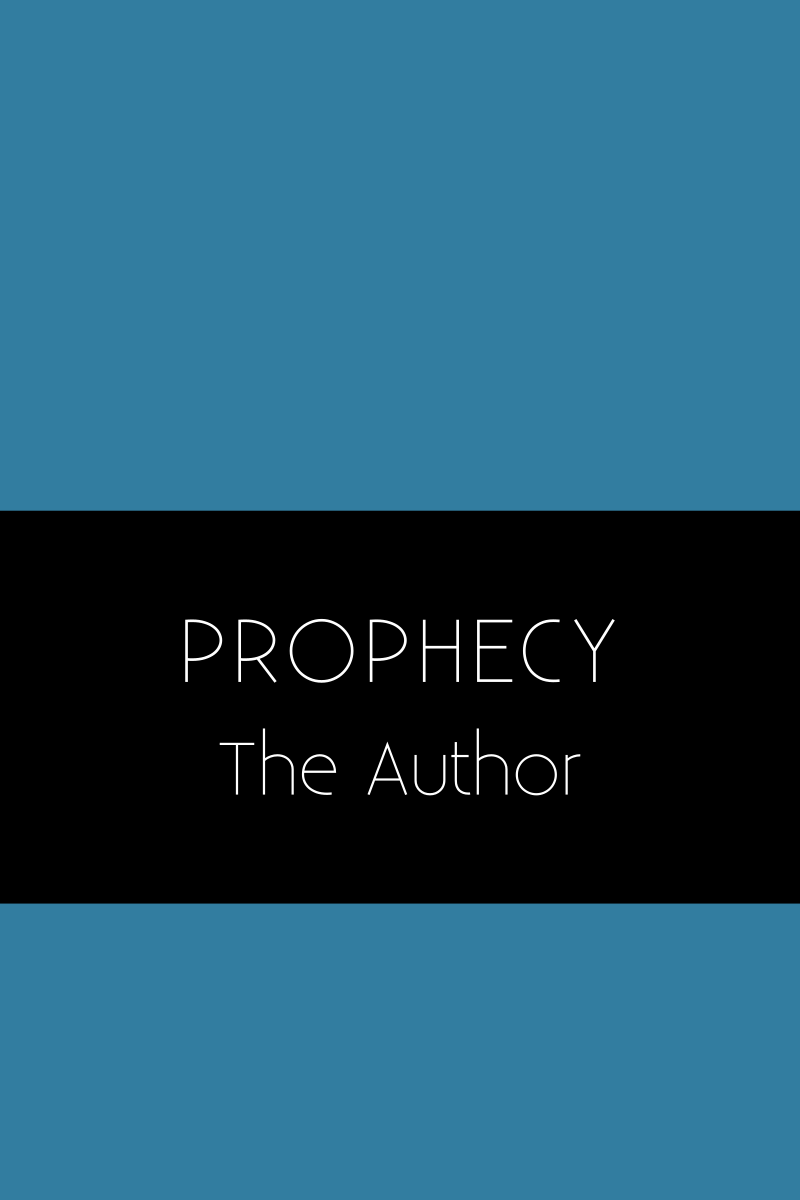
\includegraphics[height=\paperheight]{./desktop-cover.png}}
\fi

\cleartorecto
\thispagestyle{empty}
\vspace*{5em}

{\centering

\settowidth{\titleLength}{%
  {\Large\chapterTitleFont\scshape\MakeLowercase{\thetitle}}%
}

{\Large\chapterTitleFont\scshape\MakeLowercase{\thetitle}}\\[0.3\baselineskip]
\setlength{\xheight}{\heightof{X}}
\raisebox{0.5\xheight}{\color[gray]{0.4}\rule{\titleLength}{0.25pt}}\\[0.3\baselineskip]
{\itshape
\thesubtitle}

\vfill

\theauthor

\vspace*{5em}

}



\cleartoverso
\thispagestyle{empty}

{\copyrightsize
% \centering
\setlength{\parindent}{0pt}%
\setlength{\parskip}{0.8\baselineskip}%

\thetitle\\
by \theauthor

This publication is made available\\
for free distribution\\
by Aruno Publications

Aruno Publications is administered by:\\
Harnham Buddhist Monastery Trust\\
Company No. 6688355,\\
Charity Reg. No. 1126476

Contact Aruno Publications at \href{https://ratanagiri.org.uk/}{www.ratanagiri.org.uk}\\
This book is available for free download at\\
\href{https://forestsangha.org/}{www.forestsangha.org}

ISBN \theISBN

Copyright \copyright\ Aruno Publications 2021

\vfill

{\footnotesize

This work is licensed under a Creative Commons\\
Attribution-NonCommercial-NoDerivatives 4.0 International~License.

Produced with the \LaTeX\ typesetting system, set in EB Garamond,\\
Alegreya Sans and Merriweather.

% \ifdesktopversion
% \theDigitalEditionInfo
% \else
% \theEditionInfo\\
% \theDigitalEditionInfo
% \fi
\ifdesktopversion
\textit{\theDigitalEditionInfo}, 2021.
\else
\theEditionInfo\ (\theDigitalEditionInfo)
\fi

}}


\cleartorecto
\thispagestyle{empty}

\mbox{}\vfill

\begin{verse}

{\itshape
Gradually, gradually,\\
A moment at a time,\\
The wise remove their own impurities\\
As a goldsmith removes the dross.

Dhammapada v.239
}

\end{verse}

\vfill\mbox{}


\cleartorecto
\tableofcontents*

\chapter{Foreword}

Nullam eu ante vel est convallis dignissim. Fusce suscipit, wisi nec facilisis
facilisis, est dui fermentum leo, quis tempor ligula erat quis odio. Nunc porta
vulputate tellus. Nunc rutrum turpis sed pede. Sed bibendum. Aliquam posuere.
Nunc aliquet, augue nec adipiscing interdum, lacus tellus malesuada massa, quis
varius mi purus non odio. Pellentesque condimentum, magna ut suscipit hendrerit,
ipsum augue ornare nulla, non luctus diam neque sit amet urna. Curabitur
vulputate vestibulum lorem. Fusce sagittis, libero non molestie mollis, magna
orci ultrices dolor, at vulputate neque nulla lacinia eros. Sed id ligula quis
est convallis tempor. Curabitur lacinia pulvinar nibh. Nam a sapien.

\bigskip

{\raggedleft
  Reviewer Person\\
  July 2017
\par}


\chapter{Preface}

This book has been compiled in large part because dwelling on thoughts
of gratitude brings happiness. Also, as I approach seventy years of age,
I find myself drawn to recollecting and reviewing earlier events in my
life and noticing how differently I now feel about them. As the writing
of these notes progressed, it became apparent that, in addition to
gratitude, I have been reflecting on two other themes: the dynamic of
spiritual community and ways of supporting our spiritual life.

The title, `\emph{In Any Given Moment}', means two things to me. One way
of reading it reminds me that in any moment there is the potential to
let go of our painful habits of clinging and consider the larger,
spacious context in which this drama of life is taking place. This is
how I understand, `Going for refuge to the Buddha': trusting that there
is selfless, just-knowing awareness.

\enlargethispage{\baselineskip}

In another way of reading it, the cover image of an open sky (thank you
Chinch) together with the title, suggests that whether or not we notice
the beauty of life in any given moment depends on how present we are for
it. When our faculties are obscured by self-centredness, we risk
becoming lost in memories of the past and fantasies of the future; as a
result our attention readily settles on what we perceive as lacking or
`wrong' with life, and we fail to notice the goodness and beauty right
here in front of us. If our vision begins to clear, if the dross of
unawareness is gradually removed and the gold of awareness revealed, a
thoroughly different perspective might emerge.

The timeline as it is presented here should not be taken too literally.
I have tried to be accurate; however, accuracy over dates and times was
not the main point of the compilation. I apologize if any inaccuracies
or inconsistencies cause confusion. The main point has been to reflect
on gratitude, community and sustaining spiritual practice. These three
themes are the foreground, with the incidents and events of my life as
the background; sometimes the background is not quite in focus.

The significant moments that I reference in these pages, both the
positive and the negative, are moments and events that stand out as
having been helpful in my effort to be freed from the addiction to
self-centredness. By no means have all the positive influences been
mentioned, and definitely I have not included many of the negatives.
Readers will find that the first six parts of the book read somewhat like a travelogue
interspersed with Dhamma reflections. Part seven is almost
entirely Dhamma reflections. It wasn't that I set out to write a book in
this style, it is just that this is how it unfolded. My hope is that
anyone who reads it will discover something beneficial for themselves
and perhaps find something that they want to share.

\bigskip

{\raggedleft
  Ajahn Munindo
\par}



% Page 1 is the first page of the first chapter.
\mainmatter

\chapterNote{Chapter one subtitle}

\chapter{Chapter One Title}
\tocChapterNote{Chapter one subtitle}

Aliquam erat volutpat. Nunc eleifend leo vitae magna. In id erat non orci
commodo lobortis. Proin neque massa, cursus ut, gravida ut, lobortis eget,
lacus. Sed diam. Praesent fermentum tempor tellus. Nullam tempus. Mauris ac
felis vel velit tristique imperdiet. Donec at pede. Etiam vel neque nec dui
dignissim bibendum. Vivamus id enim. Phasellus neque orci, porta a, aliquet
quis, semper a, massa. Phasellus purus. Pellentesque tristique imperdiet tortor.
Nam euismod tellus id erat.


\chapterNote{Chapter two subtitle}

\chapter{Chapter Two Title}
\tocChapterNote{Chapter two subtitle}

Nullam eu ante vel est convallis dignissim. Fusce suscipit, wisi nec facilisis
facilisis, est dui fermentum leo, quis tempor ligula erat quis odio. Nunc porta
vulputate tellus. Nunc rutrum turpis sed pede. Sed bibendum. Aliquam posuere.
Nunc aliquet, augue nec adipiscing interdum, lacus tellus malesuada massa, quis
varius mi purus non odio. Pellentesque condimentum, magna ut suscipit hendrerit,
ipsum augue ornare nulla, non luctus diam neque sit amet urna. Curabitur
vulputate vestibulum lorem. Fusce sagittis, libero non molestie mollis, magna
orci ultrices dolor, at vulputate neque nulla lacinia eros. Sed id ligula quis
est convallis tempor. Curabitur lacinia pulvinar nibh. Nam a sapien.




\backmatter

\chapter{Glossary}

\begin{glossarydescription}

% === A ===

\item[anicca] (Pali) Impermanence: one of the \emph{three characteristics of
    existence} along with not-self (\emph{anattā}) and unsatisfactoriness
  (\emph{dukkha}).

% === B ===

\item[borapet] (Thai) Tinospora crispa. Heart-shaped moonseed or guduchi.
  An extremely bitter vine used as a prophylactic and treatment for malaria.

% === C ===

% === D ===

% === E ===

% === F ===

% === G ===

% === H ===

% === I ===

% === J ===

% === K ===

% === L ===

% === M ===

% === N ===

% === O ===

% === P ===

% === Q ===

% === R ===

% === S ===

% === T ===

% === U ===

% === V ===

% === W ===

\end{glossarydescription}



\cleartorecto
\thispagestyle{plain}

{\fontsize{10}{14}\selectfont%
\setlength{\parindent}{0pt}%
\raggedright\label{copyright-details}%
\setlength{\parskip}{7pt}%

{\centering

{\LARGE\ccbyncnd}

This work is licensed under a Creative Commons\\
Attribution-NonCommercial-NoDerivatives 4.0 International~License.\footnote{%
\href{https://creativecommons.org/licenses/by-nc-nd/4.0/}{https://creativecommons.org/licenses/by-nc-nd/4.0/}}

}

You are free to:

\begin{packeditemize}
\item Share — copy and redistribute the material in any medium or format
\end{packeditemize}

The licensor cannot revoke these freedoms as long as you follow the license terms.

Under the following terms:

\begin{packeditemize}
\item Attribution — You must give appropriate credit, provide a link to the license, and indicate if changes were made. You may do so in any reasonable manner, but not in any way that suggests the licensor endorses you or your use.
\item NonCommercial — You may not use the material for commercial purposes.
\item NoDerivatives — If you remix, transform, or build upon the material, you may not distribute the modified material.
\end{packeditemize}

No additional restrictions — You may not apply legal terms or technological measures that legally restrict others from doing anything the license permits.

Notices:

You do not have to comply with the license for elements of the material in the public domain or where your use is permitted by an applicable exception or limitation.

No warranties are given. The license may not give you all of the permissions necessary for your intended use. For example, other rights such as publicity, privacy, or moral rights may limit how you use the material.

% TODO confirm this notice with The Publisher

\thePublisher\ asserts its moral right to be identified as the author of this book.

\thePublisher\ requests that you attribute ownership of the work to \thePublisher\ on copying, distribution, display or performance of the work.

}


\emptyUntilEven

\end{document}
